\subsection{Interaction patterns}
The interaction between the human and the computer is depicted in Figure~\ref{fig:HCIcycles}. A distinction is made between the LEAP motion and the keyboard mouse interface. 

In the system there are several tasks that a user can perform: selecting/picking up a block, moving a block, deselecting/dropping a block, rotating view over x-axis, rotating view over y-axis. Below you will find a description of the interaction patterns for these tasks.
\newline\newline
Selecting/picking up a block: 
\newline The computer shows on the screen the environment. The user looks at the screen and finds the block that he/she wants to select. The user moves with the mouse (or hand when using the LEAP motion) to the block. The computer tracks the coordinates of the mouse/hand). When the mouse/hand is on the block the computer changes the colour of the block and shows this on the screen to the user (the blocks colour changes to light blue). The user clicks on the block using the left mouse button (or when using the LEAP motion, makes a grasp gesture). The computer recognizes this (with the LEAP motion with the gesture recognizer) and changes the colour of the block to orange.
\newline\newline
Moving a block: 
\newline The computer shows on the screen the environment. The user already has a block selected (holding the left mouse button, or for the LEAP: hand in a fist). The user moves with the mouse (or hand when using the LEAP motion). The computer tracks the coordinates of the mouse/hand) and changes the location of the block accordingly and shows this on the screen to the user. 
\newline\newline
Deselecting/dropping a block: 
\newline The computer shows on the screen the environment. The user already has a block selected (holding the left mouse button, or for the LEAP: hand in a fist). The user releases the mouse button(or when using the LEAP motion, makes an ungrasp gesture). The computer recognizes this (with the LEAP motion with the gesture recognizer). The computer drops the block on the grid and changes the colour of the block to blue.
\newline\newline
Rotating view over x-axis: 
\newline The computer shows on the screen the environment. The user presses the right/left arrow keys (or for the LEAP: makes a horizontal gesture left-to-right/right-to-left). The computer recognizes this (with the LEAP motion with the gesture recognizer). The computer changes the view accordingly.
\newline\newline
Rotating view over y-axis: 
\newline The computer shows on the screen the environment. The user presses the right/left arrow keys (or for the LEAP: makes a vertical gesture up-to-down/down-to-left). The computer recognizes this (with the LEAP motion with the gesture recognizer). The computer changes the view accordingly.

\begin{figure}[H]
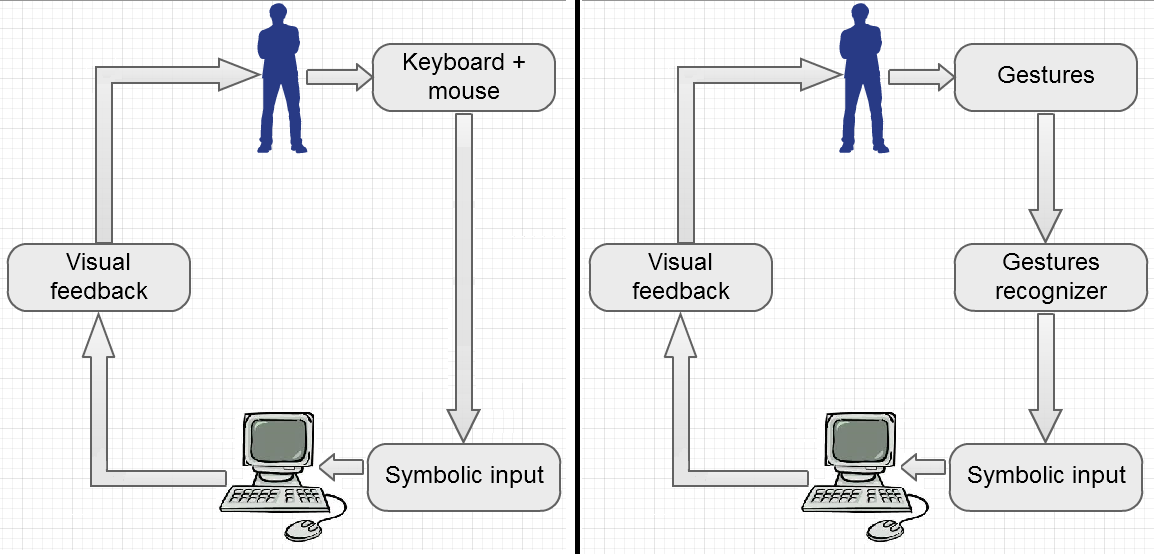
\includegraphics[width=\textwidth]{imgs/HCIcycles.png}
\caption{\label{fig:HCIcycles}HCI cycles of the interaction between the human and the computer for the two interfaces described in this paper. On the left the HCI cycle for the keyboard + mouse interface is shown and on the right the HCI cycle for the LEAP motion interface.}
\end{figure}

\subsection{Cognitive modelling}
The possible tasks of the user are modelled using the KLM-GOMS (Keystroke Level Model - Goals, Operators, Methods, and Selection rules) method~\cite{john1996goms}. The KLM-GOMS method, can be used to predict execution times. Using the KLM-GOMS method sequences of actions the user must perform to accomplish a task are specified. The estimated times needed to perform these actions are added up to predict the executions time of this particular task. It is important to keep in mind that GOMS assumes an error less performance and is generally aimed at expert users.

Card, Moran, \& Newell(1983)~\cite{card1983psychology} developed a standard set of operators (e.g. mouse click, keystroke) and their estimated execution times based on experimental data (see Table~\ref{tab:standardops}). 

The possible tasks for the user in this system are: selecting/picking up a block, moving a block, deselecting/dropping a block, rotating view over x-axis, rotating view over y-axis. The GOMS diagrams of these task can be found in Appendix D. The execution times are estimated only using the standard set of estimated execution times (see Table~\ref{tab:standardops}). Not every actions' execution time could be estimated in this way, considering that for rotating the view it depends on how much rotation the user demands. Moreover, for the LEAP motion these standards are not yet developed and predicted executions times will highly depend on implementation of gestures and expertise/training hours of the user.


\begin{table}[H]
\centering
\begin{tabular}{|l|c|}
\hline
K - keystroke & 0.28 sec\\ \hline
T(n) Type a sequence of n characters on a keyboard & n x K sec \\ \hline
P - Point with mouse to a target on the display & 1.1 sec \\ \hline
B - Press or release mouse button & 0.1 sec \\ \hline
BB - Click mouse button & 0.2 sec \\ \hline
H - Hands from keyboard to mouse or vice versa & 0.4 sec \\  \hline
M - Mental act of routine thinking or perception & 0.6 - 1.35 sec; use 1.2 sec \\ \hline
W(t) - Waiting for the system to respond & time t must be determined \\ 
\hline
\end{tabular}
\caption{\label{tab:standardops} The standard operators and estimated times for each operator considering average users.}
\end{table}

